% XCircuit output "loop_filter_sum_noise.tex" for LaTeX input from loop_filter_sum_noise.ps
\def\putbox#1#2#3{\makebox[0in][l]{\makebox[#1][l]{}\raisebox{\baselineskip}[0in][0in]{\raisebox{#2}[0in][0in]{#3}}}}
\def\rightbox#1{\makebox[0in][r]{#1}}
\def\centbox#1{\makebox[0in]{#1}}
\def\topbox#1{\raisebox{-\baselineskip}[0in][0in]{#1}}
\def\midbox#1{\raisebox{-0.5\baselineskip}[0in][0in]{#1}}
\begin{flushleft}
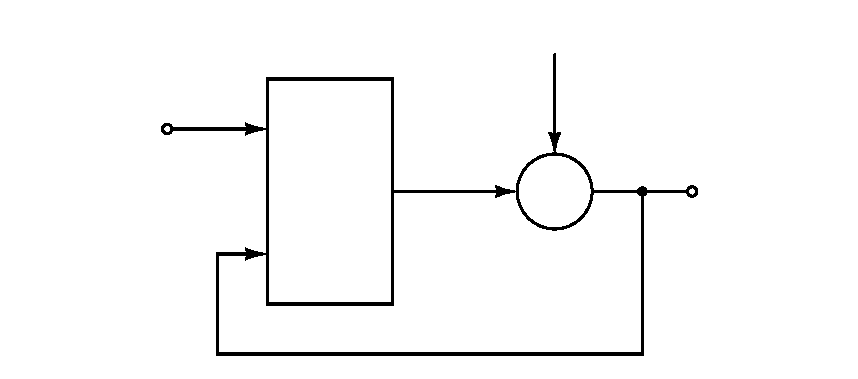
\epsfig{file=loop_filter_sum_noise.ps}\\
% translate x=590 y=416 scale 0.38
\putbox{1.88in}{1.60in}{\centbox{\midbox{$\mathcal{T}_s[\cdot]$}}}%
\putbox{1.88in}{0.76in}{\centbox{\midbox{$\mathcal{T}_n[\cdot]$}}}%
\putbox{0.75in}{1.64in}{\centbox{\midbox{\begin{small}$x(n)$\end{small}}}}%
\putbox{4.75in}{1.22in}{\centbox{\midbox{\begin{small}$y(n)$\end{small}}}}%
\putbox{2.88in}{1.31in}{\centbox{\midbox{\begin{small}$Q_{i}(n)$\end{small}}}}%
\putbox{3.59in}{1.18in}{\centbox{\midbox{$\displaystyle\sum$}}}%
\putbox{3.71in}{2.22in}{\rightbox{\midbox{$e(n)$}}}%
\end{flushleft}
